\PassOptionsToPackage{unicode=true}{hyperref} % options for packages loaded elsewhere
\PassOptionsToPackage{hyphens}{url}
%
\documentclass[]{article}
\usepackage[a4paper,top=3cm,bottom=3cm,left=3cm,right=3cm,marginparwidth=1.75cm]{geometry}
\usepackage[UTF8]{ctex}
\usepackage{lmodern}
\usepackage{amssymb,amsmath}
\usepackage{ifxetex,ifluatex}
\usepackage{fixltx2e} % provides \textsubscript
\ifnum 0\ifxetex 1\fi\ifluatex 1\fi=0 % if pdftex
  \usepackage[T1]{fontenc}
  \usepackage[utf8]{inputenc}
  \usepackage{textcomp} % provides euro and other symbols
\else % if luatex or xelatex
  \usepackage{unicode-math}
  \defaultfontfeatures{Ligatures=TeX,Scale=MatchLowercase}
\fi
% use upquote if available, for straight quotes in verbatim environments
\IfFileExists{upquote.sty}{\usepackage{upquote}}{}
% use microtype if available
\IfFileExists{microtype.sty}{%
\usepackage[]{microtype}
\UseMicrotypeSet[protrusion]{basicmath} % disable protrusion for tt fonts
}{}
\IfFileExists{parskip.sty}{%
\usepackage{parskip}
}{% else
\setlength{\parindent}{0pt}
\setlength{\parskip}{6pt plus 2pt minus 1pt}
}
\usepackage{hyperref}
\hypersetup{
            pdfborder={0 0 0},
            breaklinks=true}
\urlstyle{same}  % don't use monospace font for urls
\usepackage{color}
\usepackage{fancyvrb}
\newcommand{\VerbBar}{|}
\newcommand{\VERB}{\Verb[commandchars=\\\{\}]}
\DefineVerbatimEnvironment{Highlighting}{Verbatim}{commandchars=\\\{\}}
% Add ',fontsize=\small' for more characters per line
\newenvironment{Shaded}{}{}
\newcommand{\AlertTok}[1]{\textcolor[rgb]{1.00,0.00,0.00}{\textbf{#1}}}
\newcommand{\AnnotationTok}[1]{\textcolor[rgb]{0.38,0.63,0.69}{\textbf{\textit{#1}}}}
\newcommand{\AttributeTok}[1]{\textcolor[rgb]{0.49,0.56,0.16}{#1}}
\newcommand{\BaseNTok}[1]{\textcolor[rgb]{0.25,0.63,0.44}{#1}}
\newcommand{\BuiltInTok}[1]{#1}
\newcommand{\CharTok}[1]{\textcolor[rgb]{0.25,0.44,0.63}{#1}}
\newcommand{\CommentTok}[1]{\textcolor[rgb]{0.38,0.63,0.69}{\textit{#1}}}
\newcommand{\CommentVarTok}[1]{\textcolor[rgb]{0.38,0.63,0.69}{\textbf{\textit{#1}}}}
\newcommand{\ConstantTok}[1]{\textcolor[rgb]{0.53,0.00,0.00}{#1}}
\newcommand{\ControlFlowTok}[1]{\textcolor[rgb]{0.00,0.44,0.13}{\textbf{#1}}}
\newcommand{\DataTypeTok}[1]{\textcolor[rgb]{0.56,0.13,0.00}{#1}}
\newcommand{\DecValTok}[1]{\textcolor[rgb]{0.25,0.63,0.44}{#1}}
\newcommand{\DocumentationTok}[1]{\textcolor[rgb]{0.73,0.13,0.13}{\textit{#1}}}
\newcommand{\ErrorTok}[1]{\textcolor[rgb]{1.00,0.00,0.00}{\textbf{#1}}}
\newcommand{\ExtensionTok}[1]{#1}
\newcommand{\FloatTok}[1]{\textcolor[rgb]{0.25,0.63,0.44}{#1}}
\newcommand{\FunctionTok}[1]{\textcolor[rgb]{0.02,0.16,0.49}{#1}}
\newcommand{\ImportTok}[1]{#1}
\newcommand{\InformationTok}[1]{\textcolor[rgb]{0.38,0.63,0.69}{\textbf{\textit{#1}}}}
\newcommand{\KeywordTok}[1]{\textcolor[rgb]{0.00,0.44,0.13}{\textbf{#1}}}
\newcommand{\NormalTok}[1]{#1}
\newcommand{\OperatorTok}[1]{\textcolor[rgb]{0.40,0.40,0.40}{#1}}
\newcommand{\OtherTok}[1]{\textcolor[rgb]{0.00,0.44,0.13}{#1}}
\newcommand{\PreprocessorTok}[1]{\textcolor[rgb]{0.74,0.48,0.00}{#1}}
\newcommand{\RegionMarkerTok}[1]{#1}
\newcommand{\SpecialCharTok}[1]{\textcolor[rgb]{0.25,0.44,0.63}{#1}}
\newcommand{\SpecialStringTok}[1]{\textcolor[rgb]{0.73,0.40,0.53}{#1}}
\newcommand{\StringTok}[1]{\textcolor[rgb]{0.25,0.44,0.63}{#1}}
\newcommand{\VariableTok}[1]{\textcolor[rgb]{0.10,0.09,0.49}{#1}}
\newcommand{\VerbatimStringTok}[1]{\textcolor[rgb]{0.25,0.44,0.63}{#1}}
\newcommand{\WarningTok}[1]{\textcolor[rgb]{0.38,0.63,0.69}{\textbf{\textit{#1}}}}
\usepackage{graphicx,grffile}
\makeatletter
\def\maxwidth{\ifdim\Gin@nat@width>\linewidth\linewidth\else\Gin@nat@width\fi}
\def\maxheight{\ifdim\Gin@nat@height>\textheight\textheight\else\Gin@nat@height\fi}
\makeatother
% Scale images if necessary, so that they will not overflow the page
% margins by default, and it is still possible to overwrite the defaults
% using explicit options in \includegraphics[width, height, ...]{}
\setkeys{Gin}{width=\maxwidth,height=\maxheight,keepaspectratio}
\setlength{\emergencystretch}{3em}  % prevent overfull lines
\providecommand{\tightlist}{%
  \setlength{\itemsep}{0pt}\setlength{\parskip}{0pt}}
\setcounter{secnumdepth}{0}
% Redefines (sub)paragraphs to behave more like sections
\ifx\paragraph\undefined\else
\let\oldparagraph\paragraph
\renewcommand{\paragraph}[1]{\oldparagraph{#1}\mbox{}}
\fi
\ifx\subparagraph\undefined\else
\let\oldsubparagraph\subparagraph
\renewcommand{\subparagraph}[1]{\oldsubparagraph{#1}\mbox{}}
\fi

% set default figure placement to htbp
\makeatletter
\def\fps@figure{htbp}
\makeatother

\title{数据结构与算法I 实验9}
\author{2019201409 于倬浩}

\begin{document}

\maketitle

\hypertarget{header-n0}{%
\section{}\label{header-n0}}


\tableofcontents

\hypertarget{header-n5}{%
\subsection{一、实验内容}\label{header-n5}}

实现斐波那契堆。

额外实现了可视化。

\hypertarget{header-n12}{%
\subsection{二、核心操作\&接口}\label{header-n12}}

所有核心操作命名和算法导论保持一致。

\begin{Shaded}
\begin{Highlighting}[]
\KeywordTok{struct}\NormalTok{ node \{ }\CommentTok{//节点类}
    \DataTypeTok{bool}\NormalTok{ mark; }\CommentTok{//是否丢失过儿子}
    \DataTypeTok{int}\NormalTok{ deg; }\CommentTok{//度数}
    \DataTypeTok{int}\NormalTok{ val; }\CommentTok{//键值}
\NormalTok{    node *p, *ch, *l, *r; }\CommentTok{//父亲、儿子、左兄弟、右兄弟指针}
\NormalTok{\};}

\KeywordTok{struct}\NormalTok{ Fibonacci_Heap\{ }\CommentTok{//斐波那契堆类}
\NormalTok{    node *min; }\CommentTok{//指向根链表中最小元素}
    \DataTypeTok{int}\NormalTok{ n; }\CommentTok{//当前堆的大小}
\NormalTok{\};}

\CommentTok{// 以下方法提供给用户,内部实现涉及的其他函数不再列出。}

\KeywordTok{inline}\NormalTok{ node* fibHeapInsert(Fibonacci_Heap &h,}\DataTypeTok{int}\NormalTok{ val);}
\CommentTok{// 向堆h中插入元素val}

\KeywordTok{inline}\NormalTok{ Fibonacci_Heap fibHeapUnion(Fibonacci_Heap &a, Fibonacci_Heap &b);}
\CommentTok{// 合并堆a、b,返回新堆}
    
\KeywordTok{inline} \DataTypeTok{int}\NormalTok{ fibHeapExtractMin(Fibonacci_Heap &h);}
\CommentTok{// 提取最小元素}

\KeywordTok{inline} \DataTypeTok{void}\NormalTok{ fibHeapDecreaseKey(Fibonacci_Heap &h, node *x, }\DataTypeTok{int}\NormalTok{ val);}
\CommentTok{// 减小指定节点的数据}

\KeywordTok{inline} \DataTypeTok{void}\NormalTok{ fibHeapDelete(Fibonacci_Heap &h, node *key);}
\CommentTok{// 删除节点}
\end{Highlighting}
\end{Shaded}

\hypertarget{header-n22}{%
\subsection{三、算法设计}\label{header-n22}}

所有功能均按照算法导论给出的方法实现。

\begin{itemize}
\item
  插入

  直接将当前元素当作根,插入根链表,单次操作运行时间\(\Theta(1)\)。

\begin{Shaded}
\begin{Highlighting}[]
\NormalTok{node* fibHeapInsert(Fibonacci_Heap &h,}\DataTypeTok{int}\NormalTok{ val) \{}
\NormalTok{    node *x = }\KeywordTok{new}\NormalTok{ node; }\CommentTok{//新建节点}
\NormalTok{    x->p = x->ch = null, x->l = x->r = x;}
\NormalTok{    x->deg = }\DecValTok{0}\NormalTok{, x->val = val, x->mark = }\KeywordTok{false}\NormalTok{;}
\NormalTok{    ++h.n;}
    \ControlFlowTok{if}\NormalTok{(h.min == null) h.min = x; }\CommentTok{//根链表为空}
    \ControlFlowTok{else}\NormalTok{ \{ }\CommentTok{// 插入根链表}
\NormalTok{        x->l = h.min, x->r = h.min->r;}
\NormalTok{        h.min->r->l = x, h.min->r = x;}
        \ControlFlowTok{if}\NormalTok{(x->val < h.min->val) h.min = x;}
\NormalTok{    \}}
    \ControlFlowTok{return}\NormalTok{ x;    }
\NormalTok{\}}
\end{Highlighting}
\end{Shaded}
\item
  合并堆

  类似插入操作,由于根链表是双向链表,因此可以用\(\Theta(1)\)的运行时间拆开再合并两个链表,最后维护一下\texttt{h.min}即可,依旧很懒。

\begin{Shaded}
\begin{Highlighting}[]
\NormalTok{Fibonacci_Heap fibHeapUnion(Fibonacci_Heap &a, Fibonacci_Heap &b) \{}
    \ControlFlowTok{if}\NormalTok{(a.min == null) }\ControlFlowTok{return}\NormalTok{ b; }\ControlFlowTok{if}\NormalTok{(b.min == null) }\ControlFlowTok{return}\NormalTok{ a;}
\NormalTok{    Fibonacci_Heap ret;}
\NormalTok{    ret.min = a.min;}
\NormalTok{    node *p1 = a.min->r, *p2 = b.min->l; }\CommentTok{//合并根链表}
\NormalTok{    a.min->r = b.min, b.min->l = a.min;}
\NormalTok{    p1->l = p2, p2->r = p1;}
    \ControlFlowTok{if}\NormalTok{(b.min->val < a.min->val) ret.min = b.min; }\CommentTok{//维护min}
\NormalTok{    ret.n = a.n + b.n;}
    \ControlFlowTok{return}\NormalTok{ ret;}
\NormalTok{\}}
\end{Highlighting}
\end{Shaded}
\item
  提取最小元

  首先判断操作是否非法,即堆是否为空。接下来,把\texttt{h.min}的所有儿子放到根链表中,并把\texttt{h.min}从根链表中删除。

  之后,再使用\texttt{Consolidate}维护堆性质即可。

  \texttt{Consolidate}的大致做法是,维护一个数组,存储各种度数的节点,如果发现度数重复的就合并为度数+1的,直到整个森林没有两棵树度数相同即可。最后,再把这个数组拉成一条链,构成堆的根链表。

  代码见下:

\begin{Shaded}
\begin{Highlighting}[]
\KeywordTok{inline} \DataTypeTok{void}\NormalTok{ Consolidate(Fibonacci_Heap &h) \{}
\NormalTok{    node **a = }\KeywordTok{new}\NormalTok{ node*[h.n + }\DecValTok{1}\NormalTok{]; }\CommentTok{//维护各种度数的根}
    \ControlFlowTok{for}\NormalTok{(}\DataTypeTok{int}\NormalTok{ i = }\DecValTok{0}\NormalTok{; i <= h.n; ++i) a[i] = null;}
\NormalTok{    node *x = h.min, *end = h.min;}
    \DataTypeTok{int}\NormalTok{ cnt = }\DecValTok{0}\NormalTok{;}
    \ControlFlowTok{do}\NormalTok{\{ }\CommentTok{//统计有多少个根,并把根放入一个单独的数组,用来和修改后的区分}
\NormalTok{        ++cnt;}
\NormalTok{        x = x->r;}
\NormalTok{    \}}\ControlFlowTok{while}\NormalTok{(x != end);}
\NormalTok{    node **rootList = }\KeywordTok{new}\NormalTok{ node*[cnt];}
\NormalTok{    x = h.min, end = h.min, cnt = }\DecValTok{0}\NormalTok{;}
    \ControlFlowTok{do}\NormalTok{\{}
\NormalTok{        rootList[cnt++] = x;}
\NormalTok{        x = x->r;}
\NormalTok{    \}}\ControlFlowTok{while}\NormalTok{(x != end);}
    \ControlFlowTok{for}\NormalTok{(}\DataTypeTok{int}\NormalTok{ i = }\DecValTok{0}\NormalTok{; i < cnt; ++i) \{ }\CommentTok{//枚举每个原根链表中的节点}
\NormalTok{        x = rootList[i];}
        \DataTypeTok{int}\NormalTok{ d = x->deg;}
        \ControlFlowTok{while}\NormalTok{(a[d] != null) \{ }\CommentTok{//合并与当前节点度数相同的,直到不能合并}
\NormalTok{            node *y = a[d];}
            \ControlFlowTok{if}\NormalTok{(x->val > y->val) \{}
\NormalTok{                node *tmp = x;}
\NormalTok{                x = y, y = tmp;}
\NormalTok{            \}}
\NormalTok{            fibHeapLink(h, y, x);}
\NormalTok{            a[d] = null;}
\NormalTok{            ++d;}
\NormalTok{        \}}
\NormalTok{        a[d] = x;}
\NormalTok{    \}}
\NormalTok{    h.min = null;}
    \ControlFlowTok{for}\NormalTok{(}\DataTypeTok{int}\NormalTok{ i = }\DecValTok{0}\NormalTok{; i <= h.n; ++i) \{ }\CommentTok{//维护新的根链表}
        \ControlFlowTok{if}\NormalTok{(a[i] != null) \{}
            \ControlFlowTok{if}\NormalTok{(h.min == null) \{}
\NormalTok{                h.min = a[i];}
\NormalTok{                h.min->l = h.min->r = h.min;}
\NormalTok{            \}}
            \ControlFlowTok{else}\NormalTok{ \{}
\NormalTok{                h.min->l->r = a[i], a[i]->l = h.min->l;}
\NormalTok{                a[i]->r = h.min, h.min->l = a[i];}
                \ControlFlowTok{if}\NormalTok{(a[i]->val < h.min->val) h.min = a[i];}
\NormalTok{            \}}
\NormalTok{        \}}
\NormalTok{    \}}
    \KeywordTok{delete}\NormalTok{ a; }\CommentTok{//释放空间 防止内存泄漏}
    \KeywordTok{delete}\NormalTok{ rootList;}
\NormalTok{\}}
\end{Highlighting}
\end{Shaded}
\item
  减小键值

  先处理不合法的情况,修改键值。接下来判断是否违反了堆性质,如果违反了就递归祖先节点,维护每个节点的\texttt{mark}即可,具体操作依赖\texttt{Cut}和\texttt{CascadingCut},实现起来也比较简单。

\begin{Shaded}
\begin{Highlighting}[]
\DataTypeTok{void}\NormalTok{ fibHeapDecreaseKey(Fibonacci_Heap &h, node *x, }\DataTypeTok{int}\NormalTok{ val) \{}
    \ControlFlowTok{if}\NormalTok{(val > x->val) }\CommentTok{// 输入不合法}
        \ControlFlowTok{throw} \BuiltInTok{std::}\NormalTok{runtime_error(}\StringTok{"New key is greater than current key"}\NormalTok{);}
\NormalTok{    x->val = val; }\CommentTok{//修改键值}
\NormalTok{    node *y = x->p;}
    \ControlFlowTok{if}\NormalTok{(y != null && y->val > x->val) \{ }\CommentTok{//需要修改祖先节点的情况}
\NormalTok{        Cut(h, x, y);}
\NormalTok{        CascadingCut(h, y);}
\NormalTok{    \}}
    \ControlFlowTok{if}\NormalTok{(x->val < h.min->val) h.min = x; }\CommentTok{//维护min}
\NormalTok{\}}
\end{Highlighting}
\end{Shaded}
\item
  删除节点\\
  将指定的节点\texttt{Decrease-Key}成最小的,接下来\texttt{Extract-Min}即可。
\end{itemize}

\hypertarget{header-n104}{%
\subsection{四、测试\&可视化}\label{header-n104}}

造了一个30次操作的操作序列,并把结果做成了动图\texttt{result.gif};堆的核心代码见\texttt{fib.hpp},测试代码见\texttt{fib.cpp}。

和之前的实验一样,为了更好地观察数据结构本身的性质以及方便调试,实现了一个可视化函数\texttt{dottify()},使用开源软件包\texttt{GraphViz}渲染图像。

对于测试程序,支持\texttt{Insert,\ Extract-Min,\ Decrease-Key}。由于其他的几个操作都依赖这三个操作,因此检测了这三个操作的正确性,其他操作的正确性也就得到保证。

下面粘贴几张静态的测试结果:

\begin{figure}
\centering
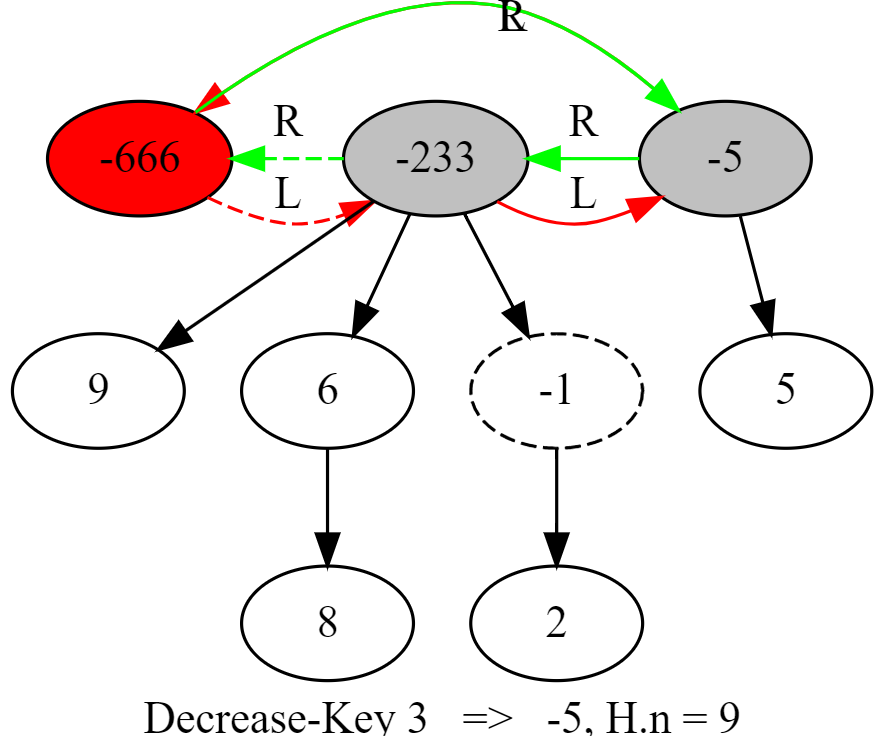
\includegraphics{C:/Users/zhuoh/Desktop/Docs/ds-lab9/Lab9_2019201409于倬浩.assets/image-20201220232156659.png}
\caption{一个操作序列对应的结果,上次操作是Decrease-Key}
\end{figure}

红色节点表示当前\texttt{h.min},灰色节点表示根列表中的点,白色节点表示非根节点,边缘带虚线的表示\texttt{mark}为\texttt{true}的节点,红绿色的边表示根链表,对于其他节点为了简洁起见,直接画出节点之间的关系,省略了链表。

具体交互方法如下:

\begin{figure}
\centering
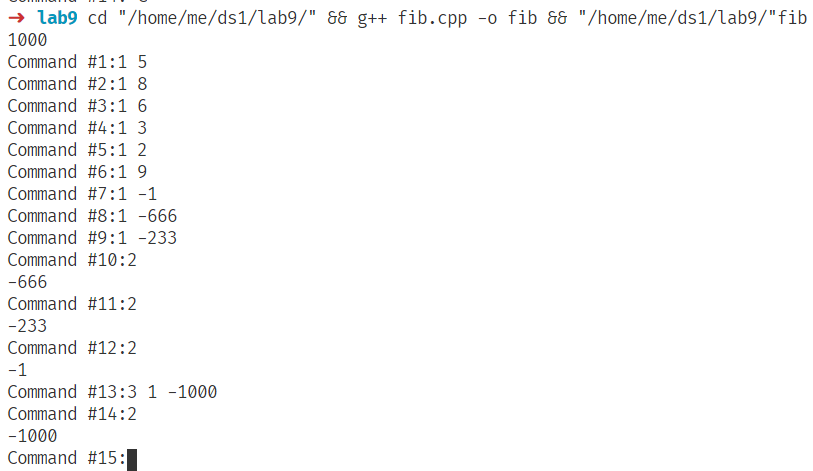
\includegraphics{C:/Users/zhuoh/Desktop/Docs/ds-lab9/Lab9_2019201409于倬浩.assets/image-20201220232724111.png}
\caption{命令行交互方法}
\end{figure}

观察操作序列对应每个时刻堆的形态,即可确定算法的正确性。

\end{document}
